\section{Approach}
\label{sec:appr}

This section describes problems with using \unsafe{} that we identified, as well as information on how to exploit these issues in the wild.
Furthermore, we present our two novel tools, \toolUsage{} and \toolSA{}, that aid in locating, evaluating and fixing potentially dangerous unsafe usages in source code.

\subsection{Usage and Security Problems}

In the following, we discuss potential threat models and exploit vectors against real-world \unsafe{} Go code.
We discuss a code pattern that is used very commonly in popular open-source Go projects as our study shows.
Listing~\ref{lst:string-to-bytes} shows how \texttt{unsafe.Pointer} is used convert a string to a \texttt{reflect.StringHeader} type.
Then, a \texttt{reflect.SliceHeader} instance is created and its fields are filled by copying the respective values from the string header.
Finally, the slice header object is converted into an actual slice of type \texttt{[]byte}.
In Go, strings are essentially read-only byte slices, and slices are represented internally by a data structure that contains its current length, allocated capacity, and memory address of the actual underlying data array.
The \texttt{reflect} header structures provide access to the internal representation.

\begin{lstlisting}[language=Golang, label=lst:string-to-bytes, caption=Common Usage of Unsafe: Conversion from String to Bytes]
func StringToBytes(s string) []byte {
	strHeader := (*reflect.StringHeader)(unsafe.Pointer(&s))
	bytesHeader := reflect.SliceHeader{
		Data: strHeader.Data,
		Cap:  strHeader.Len,
		Len:  strHeader.Len,
	}
	return *(*[]byte)(unsafe.Pointer(&bytesHeader))
}
\end{lstlisting}


\subsubsection*{Implicit Read-Only}

The conversion pattern shown in Listing~\ref{lst:string-to-bytes} is efficient as it casts between \texttt{string} and \texttt{[]byte} in-place, without the need of reallocating the slice.
Using \texttt{bytes := ([]byte)(s)} for the conversion would make the compiler allocate new memory for the slice header describing \texttt{bytes} as well as the underlying data array.
However, this pattern creates an implicitly read-only byte slice that can cause problems later on.

The Go compiler will place strings into a constant data section of the resulting binary file.
Therefore, when the binary is loaded into memory the \texttt{Data} field of the string header may contain an address that is located on a read-only memory page.
Because of this, strings are immutable by design in Go.
Mutating a string will cause a compiler error, alerting developers early in the development process that there is a problem.
However, when casting the string to a \texttt{[]byte} slice in-place, the resulting slice loses the explicit read-only property and thus the compiler will not complain about mutating this slice although the program will crash if done so.
Using this pattern therefore creates a trade-off between performance and development complexity because there are potential bugs crashing the program that can be very hard to debug if the slice resulting from this conversion gets passed around.


\subsubsection*{Garbage Collector Race}

Go uses a concurrent mark-and-sweep garbage collector to free unused memory.
It is triggered by a certain increase of heap memory usage or after some time, and runs in multiple parallel Goroutines.
The garbage collector treats pointer types, \texttt{unsafe.Pointer} values, and slice and string headers that belong to actual strings and slices as references and will mark those references as still in use, preventing them from being freed.
Importantly, \texttt{uintptr} values and string or slice headers that are created manually are not treated as references.
The last point, although documented with the \texttt{unsafe} package, is a major pitfall.
It requires that values in memory that are only reachable by converting an address stored only in a \texttt{uintptr} variable to a pointer type be treated as potentially gone.
Such cast operations create potentially dangling pointers because the memory at that address might have already been freed if the garbage collector was triggered right before the conversion.

Although not directly obvious, Listing~\ref{lst:string-to-bytes} contains such a condition.
Because the \texttt{reflect.SliceHeader} value is created as a composite literal instead of being derived from an actual slice value, its \texttt{Data} field is not treated as a reference if the garbage collector runs between lines 3 and 8, and thus the underlying data array of the resulting \texttt{[]byte} slice after the conversion might have already been collected.
This creates a potential use-after-free or buffer reuse condition that, even worse, is triggered non-deterministically when the garbage collector runs at just the right time.
Therefore, it is a race condition that can crash the program or even be an information leak vulnerability.
If the buffer is reused after being freed and the resulting slice after the cast is pointing to it, it might provide access to completely unrelated data even in concurrent Goroutines, and this has serious security implications if the resulting slice is read back to a user.

\begin{figure}[!t]
    \vspace{2mm}
    \centering
    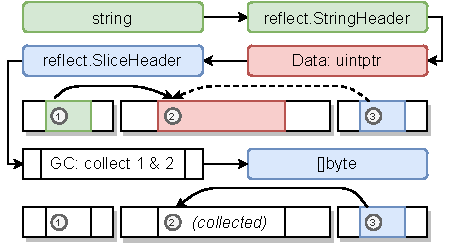
\includegraphics[width=0.4\textwidth]{gfx/figures/gcrace-vuln.pdf}
    %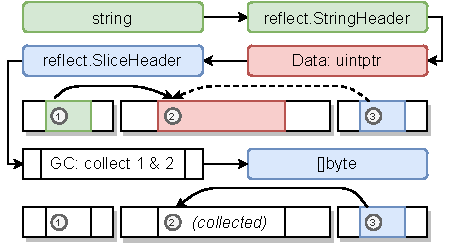
\includegraphics[width=0.48\textwidth]{gfx/figures/gcrace-vuln.pdf}
    \caption{GC race and escape analysis flaw}
    \label{fig:gcrace-vuln}
    \vspace{-8pt}
\end{figure}


Figure~\ref{fig:gcrace-vuln} shows a visualization of the casting process that leads to the problems described here.


\subsubsection*{Escape Analysis Flaw}

A third problem with the casting pattern shown in Listing~\ref{lst:string-to-bytes} is that the escape analysis algorithm can not infer a connection between the string parameter \texttt{s} and the resulting byte slice.
Although they use the same underlying data array, the algorithm misses this due to the fact that the intermediate representation as \texttt{uintptr} variable is not treated as a reference type.
This can cause the program to have undefined behavior if the returned value from the casting function is used incorrectly.

Listing~\ref{lst:escape-analysis} shows a simple program that uses the common conversion function of Listing~\ref{lst:string-to-bytes}.
In the \texttt{main} function, \texttt{GetBytes} is called which creates a string and converts it into a bytes slice using the unsafe cast.
The string is created using a \texttt{bufio} reader so that it is not constant and thus placed into the constant section of the binary, but it could also be user-provided input.
After the cast, \texttt{GetBytes} prints the resulting bytes and returns it back to \texttt{main}, which also prints the bytes.
Although one would assume that both print statements result in the string to be printed, the second one in \texttt{main} fails and prints invalid data.

\begin{lstlisting}[language=Golang, label=lst:escape-analysis, caption=Escape Analysis Flaw]
func main() {
	bytesResult := GetBytes()
	fmt.Printf("main: %s\n", bytesResult) // expected (but failed) stdout is "abcdefgh
}

func GetBytes() []byte {
	reader := bufio.NewReader(strings.NewReader("abcdefgh"))
	s, _ := reader.ReadString('\n')
	out := StringToBytes(s)
	fmt.Printf("GetBytes: %s\n", out) // expected stdout is "abcdefgh"
	return out
}
\end{lstlisting}

The reason for this is that when the string \texttt{s} is allocated in \texttt{GetBytes}, Go escape analysis will try to figure out if it escapes.
It finds that \texttt{s} is passed to \texttt{StringToBytes} and the escape analysis transitively looks into that function, where it fails to connect \texttt{s} to the returned byte slice as described above.
Therefore, escape analysis finds that \texttt{s} s does not escape in \texttt{StringToBytes}, and because it is not used after that call in \texttt{GetBytes}, the algorithm incorrectly assumes that it does not escape at all and places \texttt{s} on the stack.
When \texttt{GetBytes} prints the resulting slice, the data is still valid and the correct data is printed, but when \texttt{GetBytes} returns to \texttt{main}, its stack is destroyed.
\texttt{bytesResult} in \texttt{main} now is a dangling pointer into the former stack of \texttt{GetBytes} and therefore printing the bytes accesses invalid data.


\subsubsection*{Correct In-Place Cast}

To avoid the problems described in the previous sections, it is crucial to not create instances of \texttt{reflect.SliceHeader} and \texttt{reflect.StringHeader} from scratch, instead they must be derived from actual slices or strings.
Although this is documented with the \texttt{unsafe} package, there are many incorrect usages in the projects we analyzed.
A correct version of the in-place cast is shown in Listing~\ref{lst:correct-slice-cast}.

\begin{lstlisting}[language=Golang, label=lst:correct-slice-cast, caption=Correct In-Place String to Bytes Cast]
func StringToBytes(s string) (b []byte) {
	strHeader := (*reflect.StringHeader)(unsafe.Pointer(&s))
	bytesHeader := (*reflect.SliceHeader)(unsafe.Pointer(&b))
	bytesHeader.Data = strHeader.Data
	bytesHeader.Cap = strHeader.Len
    bytesHeader.Len = strHeader.Len
	return
}
\end{lstlisting}


\subsubsection*{Potential Code Execution}

To show further potential for real threats using \unsafe{}, we created a proof of concept for a code execution exploit using Return Oriented Programming (ROP) on a vulnerability caused by a misuse of \unsafe{}.
The vulnerability causes a buffer overflow, and since Go programs are typically statically linked with a big runtime, ASLR is not effective and there is a large number of gadgets available.
Since including the proof of concept in this paper would be too long, we put it along with other exploit demonstrations into a repository on GitHub\footnote{\url{https://github.com/jlauinger/go-unsafepointer-poc}}. 


\subsection{\toolSA{}: An Unsafe-focused Linter for Developers}

This section presents \toolSA{}, a novel static code analysis tool to find two usage patterns that were previously uncaught with existing tools.

\subsubsection*{Design}

Figure~\ref{fig:safer-architecture} shows an overview of the architecture of \toolSA{}.
\toolSA{} build upon the infrastructure provided by the Go Vet tool, which allows to add new static code analysis passes that can depend on existing ones, without having to build the CLI and output logic as well as package parsing.

\begin{figure}[!t]
    \vspace{2mm}
    \centering
    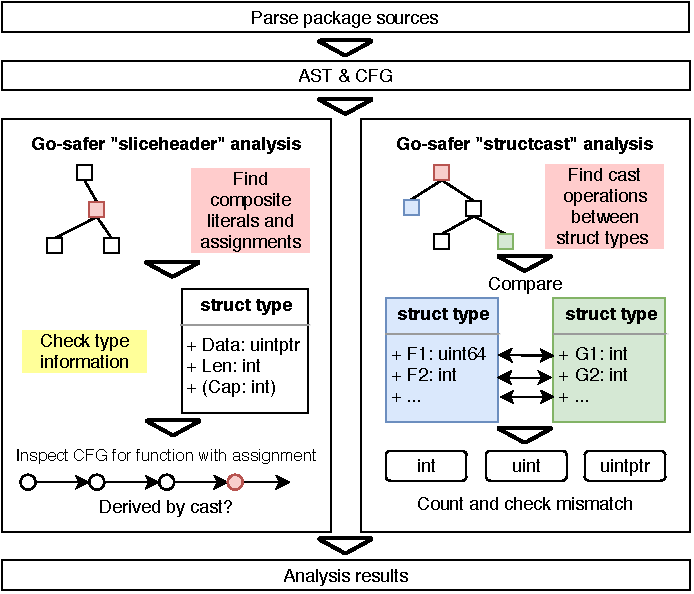
\includegraphics[width=0.48\textwidth]{gfx/figures/go-safer-architecture.pdf}
    %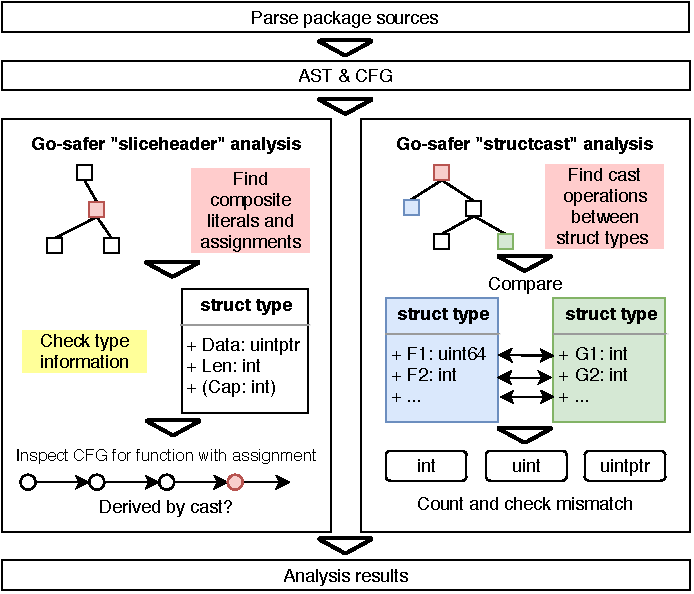
\includegraphics[width=0.45\textwidth]{gfx/figures/go-safer-architecture.pdf}
    \caption{Architecture of \toolSA{} static code analysis tool}
    \label{fig:safer-architecture}
    %\vspace{-14pt}
\end{figure}


%% put this here to manually position the figure one page earlier. Belongs to the next section (go-geiger), reposition if needed.
\begin{figure}[htp!]
    %\vspace{2mm}
    \centering
    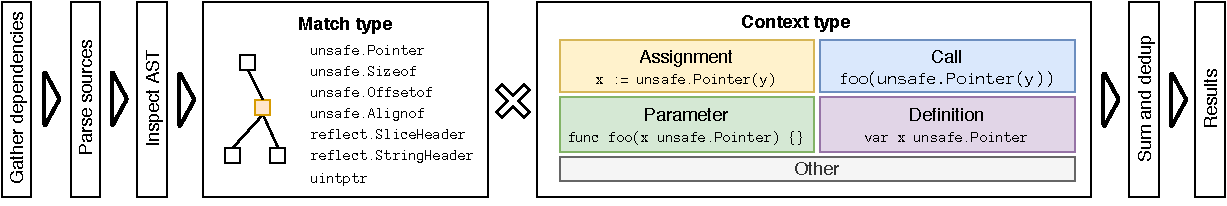
\includegraphics[width=\textwidth]{assets/figures/chapter4/go-geiger-architecture.pdf}
    \caption{Architecture of the \toolGeiger{} tool to detect unsafe usages}
    \label{fig:geiger-architecture}
    %\vspace{-10pt}
\end{figure}



\subsubsection*{Implementation}

We contribute two different novel passes: \textit{sliceheader} and \textit{structcast}.
The \textit{sliceheader} pass finds \texttt{*ast.CompositeLit} nodes in the abstract syntax tree (AST) and determines whether their type is \texttt{reflect.StringHeader}, \texttt{reflect.SliceHeader} or some derived type with the same signature.
Furthermore, it finds \texttt{*ast.AssignStmt} nodes representing assignments to variables of such types.
If it finds any, it looks up the assignment statement in the control flow graph of the corresponding function, tracks back the most recent definition of the header variable and determines whether it was derived by a cast.
If it can not certainly infer that it was in fact cast from a real slice or string, the tool will issue a warning.
The \textit{structcast} pass finds instances of in-place casts between different struct types, where the types contain an unequal amount of fields with types \texttt{int}, \texttt{uint}, or \texttt{uintptr}.
These fields have architecture-dependent sizes and offsets, and therefore casting between them might work on one architecture but break on other architectures or with different of future compilers, thus creating a risk of bugs that can crash the program or lead to invalid results on a target platform while still working fine on the developer's platform.


\subsection{\toolUsage{}: Automatic Identification of Unsafe Usage}

This section presents \toolUsage{}, a novel tool to identify and count usages of \unsafe{} in a package and its dependencies.
The project is inspired by \textit{Cargo Geiger}\footnote{\url{https://github.com/rust-secure-code/cargo-geiger}}, a similar tool for detecting unsafe code blocks in Rust programs.

\subsubsection*{Design}

Figure~\ref{fig:geiger-architecture} shows an overview of the architecture of \toolUsage{}.
We use the parsing infrastructure provided by Go to parse packages and their dependencies.
In particular, we use the \texttt{packages.Load} function to parse packages, and the \texttt{ast.Inspect} function to facilitate analysis of the abstract syntax tree (AST).
Then, we identify different usages of \unsafe{} and their context as described in the next paragraph.
Finally, we arrange the packages requested for analysis and their dependencies as an import tree and count unsafe usages for each package on its own as well as including its dependencies, taking care of proper deduplication if the same package is transitively imported more than one time.

\subsubsection*{Implementation}

We detect all usages of methods and fields from the \texttt{unsafe} package, that is \texttt{Pointer}, \texttt{Sizeof}, \texttt{Offsetof}, and \texttt{Alignof}.
Furthermore, because they often participate in unsafe operations, we also count occurrences of \texttt{reflect.SliceHeader}, \texttt{reflect.StringHeader}, and \texttt{uintptr}.
All of these usages are referred to as \unsafe{} usages in this paper.
\jl{This should probably be made clear earlier?}

The first six \unsafe{} types are detected by finding \texttt{*ast.SelectorExpr} nodes with matching field names, while \texttt{uintptr} usages are found be inspecting \texttt{*ast.Ident} nodes.
In addition, we determine the context in which the \unsafe{} usage is found as either in an assignment (classified as having a \texttt{*ast.AssignStmt}, \texttt{*ast.CompositeLit}, or \texttt{*ast.ReturnStmt}) further up in the AST, as part of a call to a function (\texttt{*ast.CallExpr}), as a function parameter declaration in the function definition (\texttt{*ast.FuncType}), a general variable definition (\texttt{*ast.GenDecl}), or other.

\todo{Switch Order of go-geiger and go-safer?}